
\documentclass[article]{memoir}

\usepackage{graphicx}
\pagestyle{empty}

\begin{document}

\chapter*{Figures \& Graphics}

Using pdf\LaTeX{} gives us more flexibility with image formats. Any image format may be used, as long as it's one of PDF, JPG or PNG---and any image you have can be losslessly converted to one of these three. A brief description of the file types:

\begin{enumerate}
  \item{PDF graphics are best used for vector diagrams; see Figure~\ref{fig:pdf} for an example;}
  \item{PNG graphics are lossless raster images used for precise bitmap images; see Figure~\ref{fig:png} for an example.}
  \item{JPG graphics are compressed bitmaps usually used for photos; see Figure~\ref{fig:jpg} for an example;}
\end{enumerate}

Figures are placed as floats, so that \LaTeX\ can place them in the most appropriate place in your document. The \verb|\includegraphics| command is what places the graphic.

\begin{figure}[hbtp]
  \centering 
  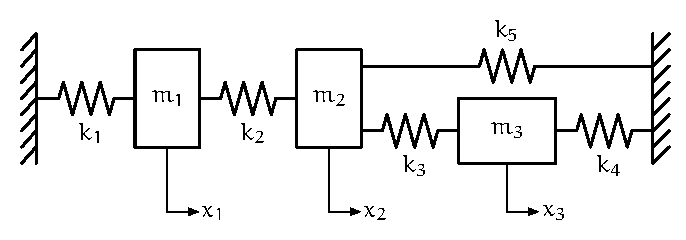
\includegraphics[width=0.9\textwidth]{./pdf-example}
%  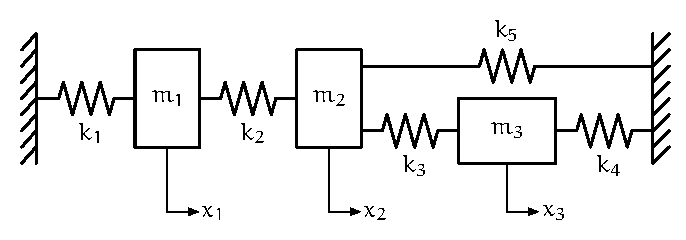
\includegraphics[width=5\textwidth]{./pdf-example} % for a really big version!
  \caption{An example PDF diagram. It can be infinitely re-scaled without loss of quality while retaining a small file size (try it and see!).}
  \label{fig:pdf}
\end{figure}

See the document ``Using imported graphics in \LaTeX{}''\footnotemark for more information. It refers only to EPS files, but the information it has is still accurate. It was written before pdf\TeX{} but the techniques it covers are still 100\% relevant. If you actually \emph{want} to include EPS figures, use the \textsf{epstopdf} package, which will convert them on the fly as it goes.

\footnotetext{\texttt{http://www.ctan.org/tex-archive/info/epslatex.pdf} if it's not on your computer}

\begin{figure}[hbtp]
  \centering
  
\includegraphics[height=10em]{./png-example}
  \caption{An example PNG image. Useful for bitmap pictures with exact output required.}
  \label{fig:png}
\end{figure}

\begin{figure}[htbp]
  \centering
  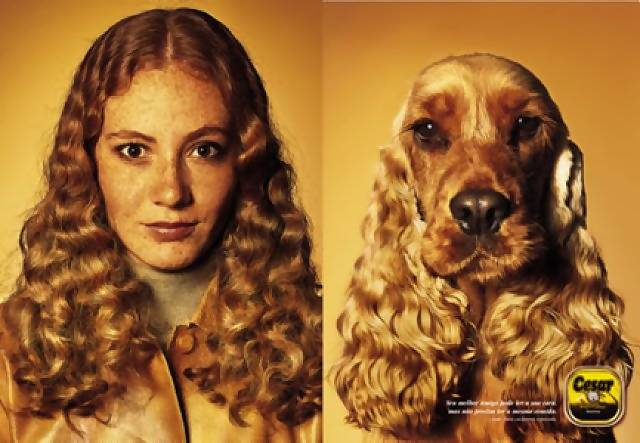
\includegraphics[scale=1.5]{./jpg-example}
  \caption{An example JPG picture. This format is good for photos because the compression is efficient but lossy.}
  \label{fig:jpg}
\end{figure}

\end{document}